\documentclass[tikz,border=3mm]{standalone}
\usepackage[utf8]{inputenc}
\usepackage[T1]{fontenc}
\usepackage{helvet}
\renewcommand{\familydefault}{\sfdefault}
\usetikzlibrary{arrows.meta,positioning}
\begin{document}

\tikzset{every node/.append style={font=\sffamily\small}}
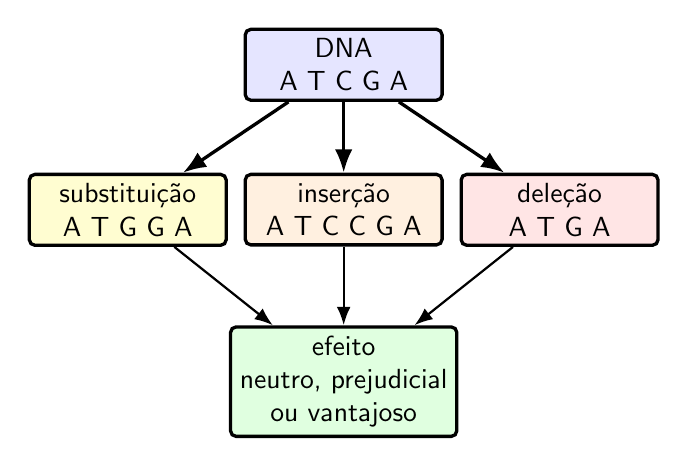
\begin{tikzpicture}[>=Latex,node distance=0.7cm]
  \tikzstyle{box}=[draw,rounded corners=2pt,very thick,align=center,minimum width=2.5cm,minimum height=0.75cm]
  \node[box,fill=blue!10] (dna) {DNA\\A T C G A};
  \node[box,fill=yellow!18,below left=0.9cm and 0.2cm of dna] (sub) {substituição\\A T G G A};
  \node[box,fill=orange!12,below=0.9cm of dna] (ins) {inserção\\A T C C G A};
  \node[box,fill=red!10,below right=0.9cm and 0.2cm of dna] (del) {deleção\\A T G A};
  \node[box,fill=green!12,below=1.0cm of ins] (efeito) {efeito\\neutro, prejudicial\\ou vantajoso};
  \draw[very thick,->] (dna) -- (sub);
  \draw[very thick,->] (dna) -- (ins);
  \draw[very thick,->] (dna) -- (del);
  \draw[thick,->] (sub) -- (efeito);
  \draw[thick,->] (ins) -- (efeito);
  \draw[thick,->] (del) -- (efeito);
\end{tikzpicture}
\end{document}
